% !TEX root = ../patchEmbeddings_review.tex
\begin{figure}[t]
\centering
\begin{minipage}[t]{0.36\textwidth}
        \centering
        % \includegraphics[width=0.4\textwidth,trim=0.25in 0.25in 0.68in 0.36in,clip]{./figs/SSBM_experiments.pdf} % 0.45
        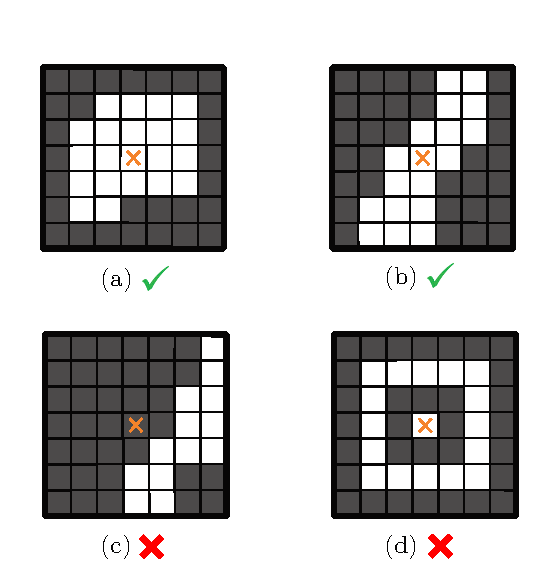
\includegraphics[width=0.99\textwidth]{./figs/valid_masks.pdf} % 0.45
        \captionof{figure}{Examples of expected and not expected binary 2D \maskname masks. Masks \textbf{(a-b)} represent two possible meaningful central instance masks. Mask \textbf{(c)} is not expected because it does not contain the central pixel. Mask \textbf{(d)} is not an expected mask because it presents more than one connected component.}
    \label{fig:valid_masks}
\end{minipage}\hfill
\begin{minipage}[t]{0.58\textwidth}
\centering
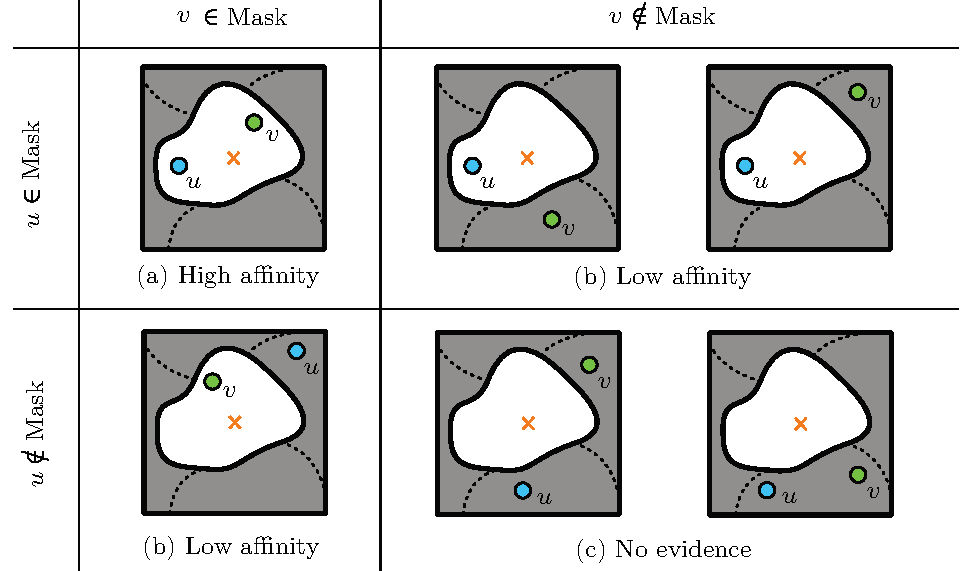
\includegraphics[width=0.99\textwidth]{./figs/mask_cases_new.pdf} % 0.45
        \captionof{figure}{Computing instance-aware affinity between pixel $u$ and $v$ (blue and green dots, respectively) from instance masks associated to the central pixel in the patch (orange cross). Dashed lines represent ground-truth boundaries separating neighboring segments. We distinguish three cases: \textbf{(a)} when both pixels are part of the mask, a high affinity between the pixels is predicted; \textbf{(b)} when only one of them is part of the mask, we predict a low affinity; \textbf{(c)} when both pixels are not part of the mask, nothing can be said about their affinity.}
    \label{fig:mask_cases}
\end{minipage}
\end{figure}

\begin{algorithm}[t]
  \begin{flushleft}
  \caption{: Affinities from Aggregated Central Instance Masks}
   \hspace*{\algorithmicindent} \textbf{Input:} Graph $\mathcal{G}(V,E)$; \maskname masks $\mathcal{M}_{\coord{u}}: \mathcal{N}_{K\times K} \rightarrow [0,1]$  \\
  \hspace*{\algorithmicindent} \textbf{Output:} Affinities $\bar{a}_e\in[0,1]$ with variance $\sigma^2_e$ for all edges $e\in E$\\
  \hspace*{\algorithmicindent} 
  \begin{algorithmic}[1]
  \footnotesize
  % \small
      % \State Initial clustering: $\Pi=\{\{v_1\}, \ldots, \{v_{|V|}\}\}$
      % \State Initialize interactions between clusters with $ = w^+_e - w^-_e$
      \For{each edge $e=(\coord{u}, \coord{v})\in E$ in graph $\mathcal{G}$}
        \State Get coordinates $\coord{u}=(u_x,u_y)$ and $\coord{v}=(v_x,v_y)$ of pixels linked by edge $e$
        \State Collect all $T$ masks $\mathcal{M}_{\coord{c}_1},\ldots,\mathcal{M}_{\coord{c}_T}$ including both pixel $\coord{u}$ and pixel $\coord{v}$
        \State Init. vectors $[a_1,\ldots,a_T] = [\evidW_1,\ldots,\evidW_T] = 0$ for affinities and evidence weights
        \For{$i\in 1, \ldots,T$}
            \State Get relative coords. of $\coord{u}$ and $\coord{v}$ with respect to the central pixel $\coord{c}_i$
            \State $a_i \gets \min \big(\mathcal{M}_{\coord{c}_i}(\coord{u} - \coord{c}_i), \,\mathcal{M}_{\coord{c}_i}(\coord{v} - \coord{c}_i)\big)$ \Comment{Fuzzy-AND: both values active}
            \State $\evidW_i \gets \max \big(\mathcal{M}_{\coord{c}_i}(\coord{u} - \coord{c}_i), \,\mathcal{M}_{\coord{c}_i}(\coord{v} - \coord{c}_i)\big)$ \Comment{Fuzzy-OR: at least one value active}
        \EndFor
        \State Get weighted affinity average $\bar{a}_e= \sum_{i} a_i \evidW_i\,/\,\sum_{i}\evidW_i$ 
        \State Get weighted affinity variance $\sigma^2_e = \sum_{i} \evidW_i (a_i-\bar{a}_e)^2\,/\,\sum_{i}\evidW_i$
      \EndFor
      \State
      \Return $\bar{a}_e, \sigma^2_e$ for each $e\in E$
  \end{algorithmic}
    \label{alg:computing_affinities}
  \end{flushleft}

\end{algorithm}
\begin{figure}[t]
\centering
        % \includegraphics[width=0.4\textwidth,trim=0.25in 0.25in 0.68in 0.36in,clip]{./figs/SSBM_experiments.pdf} % 0.45
        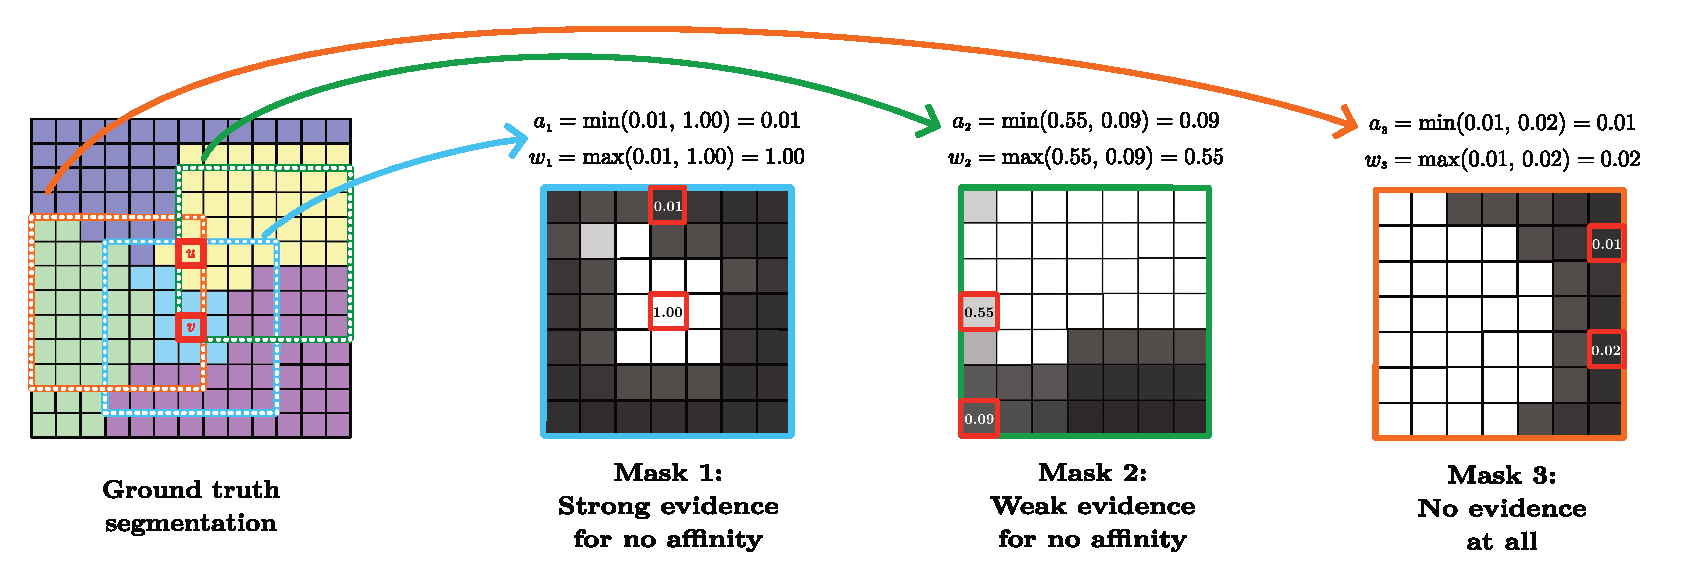
\includegraphics[width=0.9\textwidth]{./figs/mask_average_new.eps} % 0.45
        \caption{Proposed method to average overlapping masks and compute the affinity between pixel $u$ and pixel $v$ (highlighted in red in the ground-truth segmentation on the left). For simplicity, we only consider three masks among all the ones including both pixels $u$ and $v$. 
        % For each of the three masks in the lower part of the figure, we highlight in red the predicted probabilities for $u$ and $v$ to be part of the instance that covers the central pixel of the mask. 
        In \emph{Mask 1}, only $v$ is part of the mask, so there is a strong evidence for no affinity between $u$ and $v$; in \emph{Mask 2},  $u$ is predicted to be part of the mask only with a low confidence, so the contribution of this mask in the final average will be weak; in \emph{Mask 3}, both pixels are not part of the \maskname mask, so there is no evidence about their affinity. 
        The final affinity value of edge $(u,v)$ is given by the weighted average of the collected affinities $a_i$ weighted with the evidence weights $\evidW_i$: $\bar{a}_e= \sum_{i=1}^3 a_i \evidW_i\,/\,\sum_{i}\evidW_i$}
    \label{fig:alg_explained}
\end{figure}


\section{Extracting Affinities from Central Instance Masks}
In order to obtain an instance segmentation from the predictions of the model presented in Sec. \ref{sec:model}, we now compute instance-aware pixel-pair affinities for a given sparse $N$-neighborhood structure (see Table \ref{tab:neighborhood_structures} in supplementary material for details about the structure) and use them as edge weights of a pixel grid-graph $\mathcal{G}(V,E)$, such that each node represents a pixel / voxel of the image. The graph is then partitioned to obtain object instances.
% \TODO{Section intro} Second contribution; two ways
% In this section, we propose two ways to perform something similar and use the predicted per-pixel \maskname masks to define the edge weights of a grid-graph.



\subsection{Affinities with Uncertainty from Aggregated Masks}\label{sec:aggr_affs}
In this section, we propose an algorithm that, without the need of any threshold parameter, aggregates predictions from overlapping \maskname masks and outputs edge weights with associated uncertainty.
Related work either thresholds the predicted \maskname masks \cite{januszewski2018high,hirsch2020patchperpix,meirovitch2016multi} or computes Intersection over Union (IoU) scores for overlapping patches \cite{liu2016multi}. However, an advantage of predicting pixel-pair affinities / pseudo-probabilities as compared to IoU scores is that affinities can easily be translated into attractive and repulsive interactions in the grid-graph 
% i.e. edge with either positive or negative weights, 
and a parameter-free partitioning algorithm can be employed to yield instances.
% Related work in \cite{liu2016multi} aggregate \maskname masks by computing Intersection over Union (IoU) scores for overlapping patches, however these scores cannot be translated into attractive and repulsive cues of the graph, so hierarchical agglomerative clusterings 

Here, we propose a simple algorithm to aggregate predictions from multiple patches: Fig. \ref{fig:alg_explained} shows a simplified example of how Algorithm \ref{alg:computing_affinities} computes the affinity for an edge $e$ linking a pair of pixels $\coord{u}$ and $\coord{v}$.
As a first step, the algorithm loops over all predicted \maskname masks including both $\coord{u}$ and $\coord{v}$. 
% For example, if $\coord{u}$ and $\coord{v}$ are direct neighbors and the predicted masks have shape $K\times K$, then there will be $K(K-1)$ masks including both pixel $\coord{u}$ and $\coord{v}.$\footnote{Note that here we ignore possible boundary effects by considering two pixels close to the image border.} 
However, not all these masks are informative, as we visually explain in Fig.~\ref{fig:mask_cases}: a mask $\mathcal{M}_{\coord{c}_i}$ centered at pixel $\coord{c}_i$ provides any evidence about the affinity between pixels $\coord{u}$ and $\coord{v}$ only if at least one of the two pixels belongs to the mask (fuzzy OR operator at line 8 in Alg. \ref{alg:computing_affinities}).
If both pixels do note belong to it, we cannot say anything about whether they belong to the same instance (see Fig. \ref{fig:mask_cases}c). We model this with an evidence weight $\evidW_i\in[0,1]$, which is low when both pixels do not belong to the mask.
% If both pixels do not belong to it, then the evidence weight  goes to zero (see Fig. \ref{fig:mask_cases}c).
On the other hand, when at least one of the two pixels belongs to the mask, we distinguish two cases (fuzzy AND operator at line 7 in Alg. \ref{alg:computing_affinities}): i)
both pixels belong to the mask  (case in Fig. \ref{fig:mask_cases}a), so by transitivity we conclude they should be in the same instance and their affinity $a_i$ should tend to one; 
ii) only one pixel belongs to the mask (case in Fig. \ref{fig:mask_cases}b), so that according to this mask they are in different instances and their affinity should tend to zero. 

At the end, we compute a weighted average $\bar{a}_e$ and variance $\sigma^2_e$ of the collected affinities from all overlapping masks, such that masks with more evidence will contribute more on average, and the obtained variance is a measure of how consistent were the predictions across masks. 
The algorithm was implemented on GPU using PyTorch \cite{NEURIPS2019_9015} and the variance was computed via Welford's online stable algorithm \cite{welford1962note}.


\subsection{Efficient Affinities for any Sparse Neighborhood}\label{sec:efficient_affs}
An advantage of training dense \maskname masks is that the graph $N$-neighborhood structure can be defined at prediction time, after the model has been trained. As an alternative to the method presented in Sec. \ref{sec:aggr_affs} that aggregates overlapping masks, here we propose the following efficient approach to predict affinities for a sparse neighborhood structure: Given a model that has been already trained end-to-end to predict encoded \maskname masks, we stack few additional convolutional layers that are trained to convert the $Q$-dimensional latent mask space to $N$ output feature maps representing affinities for the chosen sparse neighborhood structure. These last layers are not trained jointly with the full model, so in practice they are very quick and easy to train with a binary classification loss. By using this method, we avoid to decode all masks explicitly (one for each pixel) and achieve great time and memory savings.
As a result, we obtain a model that at inference time is no more memory-consuming than the current state-of-the-art approach predicting affinities only for a specific sparse neighborhood structure.
% If the model is trained only with the \emph{\sparseBr branch} shown in Fig. \ref{fig:main_figure}a, then the desired $N$-neighborhood structure defining the connectivity of the grid-graph has to be defined before training. 
% On the other hand, if the model is trained with the \emph{\encBr branch} of Fig. \ref{fig:main_figure}c, then the sparse connectivity structure of the graph can be defined at prediction time, but the \maskDec in Fig. \ref{fig:main_figure}c has to be applied to each pixel of the image in order to predict the desired affinity values, given by the value of $N$ in each mask. 
% Alternatively, another much more efficient method consists in predicting these affinities directly from the $Q$-dimensional latent space of the encoded masks, by stacking a few additional convolutional layers that do not need to be jointly trained with the full model and only serve to convert the encoded latent space to the desired $N$ output feature maps.
% % ,  predict  from the previously trained latent space feature maps $Q\times H\times W$.
% In this way, the graph $N$-neighborhood structure can be defined at prediction time, but the resulting model is no more memory-consuming than one directly trained to predict only that specific neighborhood. 



